\begin{tikzpicture}[inner sep=4.5mm]
\node[fill, rectangle, c1] at (0,0) {};
\node[fill, rectangle, c2] at (1,0) {};
\node[fill, rectangle, c3] at (2,0) {};
\node[fill, rectangle, c4] at (3,0) {};
\node[fill, rectangle, c5] at (4,0) {};
\end{tikzpicture}

\subsection{Teor\'ia General de la Relatividad}
La cosmolog\'ia moderna se basa en la Teoría de la Relatividad General (TRG), propuesta por
Albert Einstein \citep{1917AE}, seg\'un el cual las propiedades geom\'etricas del espacio-tiempo
dependen de la distribución de materia y energ\'ia en el Universo. Dentro de TGR, las estructuras a grande escala que observamos hoy se formaron y evolucionaron (y est\'an evolucionando) a partir de 
inhomogeneidades en la distribución de masa del Universo primitivo que luego crecen bajo la influencia de la gravedad. \\

Estas ideas forman la base del \Textit{Modelo Cosmológico Estándar} ($\Lambda$-CDM\footnote{$\Lambda$-Cold Dark Matter}). \\

La Teor\'ia General de la Relatividad se basa en las \Textit{ecuaciones de campo de Einstein}:
\begin{equation}
R_{\mu \nu}-\frac{1}{2}g_{\mu \nu} R=\frac{8 \pi G}{c^4}T_{\mu \nu}-g_{\mu \nu}\Lambda,
\end{equation}
donde $R_{\mu \nu}$ (el tensor de curvatura de Ricci), $R$ (el escalar de curvatura) y $g_{\mu \nu}$ (el tensor m\'etrico) son t\'erminos relacionados con la geometr\'ia del espacio tiempo y $T_{\mu \nu}$ (el tensor de energ\'ia-esfuerzo) describe la densidad y flujo de energ\'ia y momentum en el espacio-tiempo; $c$ es la velocidad de la luz y $G$ es la constante gravitacional de Newton. El t\'ermino $\Lambda$ se llama \Textit{Constante Cosmol\'ogica} y representa la posibilidad de una densidad y presi\'on del vac\'io y/o que exista una rara forma de energ\'ia/materia gravitacional repulsiva, o Energ\'ia Oscura. \\

A partir de las mediciones de la radiaci\'on CBM, a largas escalas, el Universo puede considerarse espacialmente homeg\'eneo e isotr\'opico; en cuyo caso el tensor de energ\'ia-esfuerzo toma la forma de un fluido perfecto:

\begin{equation}
T_{\mu \nu}=(\rho + p)u_\mu u_\nu +pg_{\mu \nu},
\end{equation}

donde $\rho$ es la densidad de energ\'ia y $p$ es la presi\'on medida por un observador moviendose a 4-velocidad $u_\mu$. La densidda de energ\'ia suele escribirse como la contribuci\'on de cuatro fluidos posibles:

\begin{equation}
\rho=\sum \rho_i=\textcolor{c2}{\rho_m} + \textcolor{c5}{\rho_r} + \textcolor{c1}{\rho_\Lambda} + \textcolor{c3}{\rho_\kappa},
\end{equation}
donde $\textcolor{c2}{\rho_m}$,  $\textcolor{c5}{\rho_r}$, $\textcolor{c1}{\rho_\Lambda}$ y $\textcolor{c3}{\rho_\kappa}$ representan las contribuciones al presupuesto de densidad de energ\'ia de la materia, radiaci\'on, constante cosmol\'ogica y de la curvatura espacial, respectivamente. \\

El t\'ermino relacionado con la radiaci\'on usualmente se considera conformado por fotones CBM ($\rho_\gamma$) y neutrinos ($\rho_\nu$); mientras que la densidad de materia tiene aporte de materia bari\'onica ($\rho_{\Mbox{b}}$) y materia oscura fr\'ia ($\rho_{\Mbox{CDM}}$). \\

Una vez que se especifica el contenido de masa-energ\'ia del Universo, un modelo para la geometr\'ia del espacio-tiempo tiene que adoptarse para resolver las ecuaciones de campo de Einstein. Las m\'etrica de  Friemann-Roberson-Walker (FRW)

\begin{equation}
ds^2=-dt^2+a^2(t)\left[\frac{dr^2}{1-\kappa r^2}+r^2d\vartheta^2+r^2\sin^2\vartheta d\vartheta^2\right]
\end{equation}
es una soluci\'on exacta a las ecuaciones de campo de Einstein que describe todos los modelos isótropos, homogéneos,
uniformemente expandidos (o contra\'idos) del Universo. En la métrica FRW, $\kappa$
representa la curvatura espacial del universo y $a(t)$,  el \Textit{factor de escala}, representa la
expansi\'on relativa del universo. \\

Para un universo FRW, las ecuaciones de campo de Einstein pueden reducirse a dos ecuaciones independientes (\Textit{Ecuaciones de Friedmann}):


\begin{equation}
\frac{\dot{a}^2}{a^2}+\frac{\kappa c^2}{a^2}=\frac{8 \pi G}{3}\rho+\frac{\Lambda c^2}{3},
\end{equation}


\begin{equation}
\frac{\ddot{a}}{a}=-\frac{4 \pi G}{3} \left(\rho+\frac{3p}{c^2} \right)+\frac{\Lambda c^2}{3},
\end{equation}
donde $\dot{a}$ y $\ddot{a}$ representan la primera y segunda derivada temporal del factor de escala; respectivamente. \\

Para encontrar la evoluci\'on del factor de escala, se debe adoptar un modelo para la materia. En el caso de un universo FRW, es suficiente con establecer una \Textit{ecuaci\'on de estado}, es decir, $p=p(\rho)$; la cual puede parametrizarse como

\begin{equation}
p_i=\omega_i \rho_i c^2,
\end{equation}
donde el sub\'indice $i$ indica cada una de las posibles contribuciones al presupuesto de densidad de energ\'ia del universo. Para las componentes conocidas del Universo, $\omega_\gamma=\frac{1}{3}$, $\omega_{\Mbox{m}}=0$, $\omega_\kappa=-\frac{1}{3}$, $\omega_\Lambda=-1$ y $\omega_\nu$ est\'a en el rango $[0,\frac{1}{3}]$. \\

Si cada fluido se encuentra \Textit{desacoplado}, las ecuaciones de Friedmann se pueden combinar para expresar la evoluci\'on de la densidad de energ\'ia como
\begin{equation}
\dot{\rho_i}+3H(1+\omega_i)\rho_i,
\label{eq:ecF-d}
\end{equation}
donde $H$, el \Textit{par\'ametro de Hubble}, definido como

\begin{equation}
H\equiv H(t)\equiv \frac{da}{dt}\frac{1}{a},
\end{equation}
representa la tasa de expansi\'on del universo. El valor actual de $H$, denominado \Textit{constante de Hubble} suele normalizarse a la unidad, de manera que $H_0=H(t_0)=1$. Se acostumbra expresar la constante de Hubble en t\'ermino del \Textit{par\'ametro de Hubble adimensional} $h$, de manera que $H_0=100\, \textcolor{c1}{h} \,\mbox{km s}^{-1}\, \mbox{Mpc}^{-1},$\footnote{1 Mpc=$10^6$ pc = 3.086 $\times 10^{22}$ m. }
 y toda la incertidumbre en el valor de $H_0$ se asigna a $h$. \\
 
% 1 Mpc=$10^6$ pc = 3.086 $\times 10^{22}$ m.  \\
\citet{hubble0}

Una soluci\'on anal\'itica en el caso de que todas las componentes est\'en presentes no es posible,
pero para muchos casos de inter\'es es posible obtener soluciones anal\'iticas a la Ecuaci\'on \eqref{eq:ecF-d}.
Un resumen de tales soluciones se brinda en la Tabla 1. \\


La \Textit{densidad cr\'itica}, definida como
\begin{equation}
\rho_c\equiv \frac{3H^2}{8\pi G}
\end{equation}

es la densidad de energ\'ia que tendd\'ia un universo espacialemente plano ($\kappa=0$), sin constante cosmol\'ogica ($\Lambda=0$), con una tasa de expansi\'on $H(t)$. \\

El \Textit{par\'ametro de densidad} se define como

\begin{equation}
\Omega_i(t)\equiv \frac{\rho_i(t)}{\rho_c(t)}
\end{equation}
de donde 

\begin{equation}
\Omega=\Omega_m + \Omega_r + \Omega_\Lambda + \Omega_\kappa
\end{equation}

Un modelo cosmol\'ogico FRW se define especificando los valores de los tres par\'ametros cosmol\'ogicos $H_0$, $\Omega_{\Mbox{m}}$ y $\Omega_\Lambda$. \\

Los modelos FRW, al ser soluciones a universos homog\'eneos e isotr\'opicos, no permiten explicar la cantidad de estructuras en el universo. Para reproducir las \Textit{grandes estructuras} es necesario introducir inhomogeneidades iniciales en la densidad de energ\'ia que luego crecen bajo el efecto de la gravedad y gradientes de presi\'on en un universo en expansi\'on. Estas ``semillas'' se considera que fueron generadas a partir de fluctuaciones cu\'anticas, seguidas de una \'epoca de expansi\'on exponencial del universo temprano, denomida \Textit{inflaci\'on}. Las mediciones del CBM brindan restricciones observacionales a la forma de dichas pertubaciones iniciales de la densidad.\\

\begin{figure}
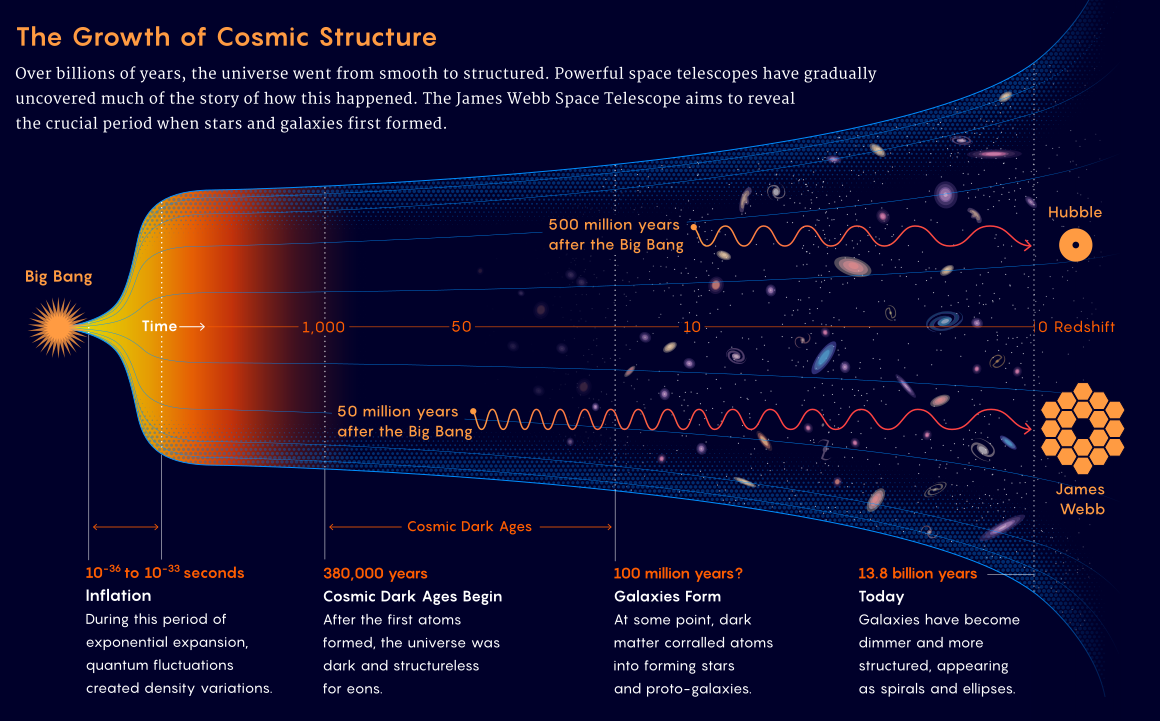
\includegraphics[width=\textwidth]{images/History-Universe-graphic.png}
\caption{El crecimiento de la estructura c\'osmica. Cr\'editos: Samuel Velasco (\href{https://www.quantamagazine.org/why-nasas-james-webb-space-telescope-matters-so-much-20211203/}{Quanta Magazine})}
\end{figure}